\documentclass[margin=3pt]{standalone}

\usepackage{tikz}
\usetikzlibrary{backgrounds, matrix, patterns}

\begin{document}

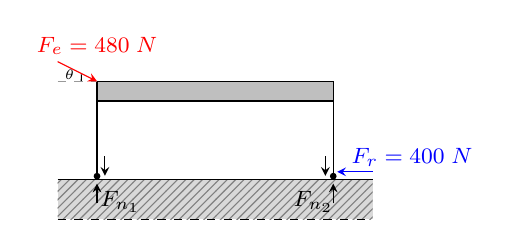
\begin{tikzpicture}
\draw (-1.7,1.75) arc (180:177:1.7) ;
\node at (-1.85,1.83) {\tiny $\theta$};

%Piso
\draw[fill=gray!30, draw=none] (-2,0) rectangle (2,0.5);
\path[pattern=north east lines, pattern color=gray] (-2,0) -- (2,0) -- (2,0.5) -- (-2,0.5) -- cycle;
\draw (-2,0.5) -- (2,0.5);
\draw[dashed] (-2,0) -- (2,0);

%Camilla
\draw (-1.5,0.5) -- (-1.5,1.5);
\draw[fill=black] (-1.5,0.545) circle (1pt);
\draw (1.5,0.5) -- (1.5,1.5);
\draw[fill=black] (1.5,0.545) circle (1pt);
\draw[fill=gray!50] (-1.5,1.5) rectangle (1.5,1.75);

%Vectores
\node[red] at (-1.5,2.2) {\footnotesize $F_{e}=480\;N$};
\draw[dashed, draw=gray!80] (-2,1.75) -- (-1.5,1.75);
\draw[red, -stealth] (-2,2) -- (-1.5,1.75);

\draw[blue, -stealth] (2,0.6) -- (1.55,0.6);
\node[blue] at (2.5,0.78) {\footnotesize $F_{r}=400\;N$};

\draw[-stealth] (1.5,0.2) -- (1.5,0.45);
\draw[-stealth] (1.4,0.8) -- (1.4,0.55);
\node[black] at (1.25,0.22) {\footnotesize $F_{n_2}$};

\draw[-stealth] (-1.5,0.2) -- (-1.5,0.45);
\draw[-stealth] (-1.4,0.8) -- (-1.4,0.55);
\node[black] at (-1.2,0.22) {\footnotesize $F_{n_1}$};
\end{tikzpicture} 


\end{document}







